\documentclass[main.tex]{subfiles}
\begin{document}
Были созданы два конвейера - тренировочный и предсказательный. Их устройство приведено на рисунке
\begin{figure}[H]
	\begin{center}
		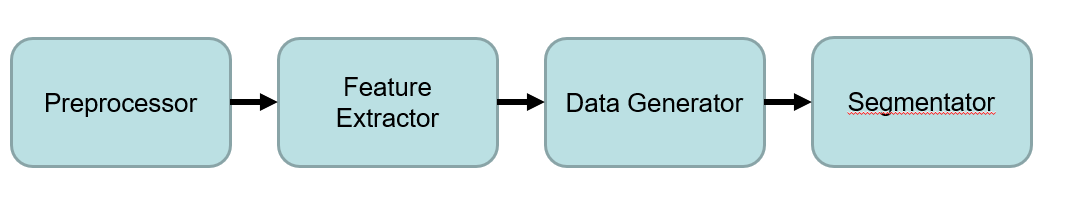
\includegraphics[scale=0.5]{images/train.png}
		\caption{Тренировочный конвейер}
	\end{center}
\end{figure}

\begin{figure}[H]
	\begin{center}
		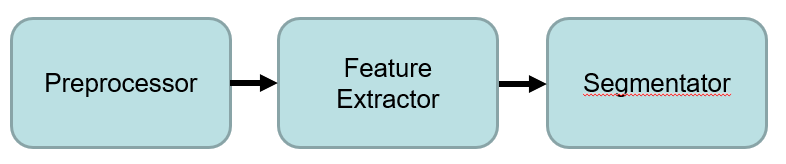
\includegraphics[scale=0.5]{images/predict.png}
		\caption{Предсказательный конвейер}
	\end{center}
\end{figure}

\subsubsection{Описание модулей}
Приведем описание каждого из модулей
\begin{itemize}
    \item Preprocessor - модуль для предобработки данных. Нужен для скачивания, конвертации видео, создания маски для видео, которые были размечены
    \item Feature Extractor - модуль для извлечения свойств(embedding) из файлов формата  .wav. В его основе архитектура VGG.
    \item Data Generator - модуль, используемый для генерации данных из AudioSet'a, а так же для некоторой предобработки данных, размеченных вручную
    \item Segmentator - модуль, в котором происходит обучение нейросети, предсказание и оценка полученных результатов
\end{itemize}

\end{document}